% =============================================================================
% APGCC 困难样本诊断 + 参考点诊断与置信度--匹配校准改进方法与实验结果(仅 A 部分)
% 依赖宏包: graphicx, booktabs, amsmath, float, multirow, tabularx
% 需 \graphicspath{{figures/}}
% =============================================================================

\subsection{APGCC困难样本诊断}

本文选择APGCC作为后续优化模型，并不是因为其在所有数据集和所有指标上均达到最优，而是因为APGCC直接输出细胞中心点，与本课题的统一点匹配评估、区域计数和错误可视化协议一致。为了明确APGCC后续应该优化什么，本文在确定APGCC为主线模型后，对其在三个统一测试集上的困难样本进行诊断分析。对每张测试图像，记真实点数为$N_i$，预测点数为$\hat{N}_i$，计数误差为$e_i=\hat{N}_i-N_i$。困难样本按照$|e_i|$排序选取，同时保留显著少计和显著多计样本；定位误差采用$12$像素半径进行一对一匹配，统计TP、FP和FN。可视化时先将图像划分为$4\times4$区域，计算每个区域的$\hat{N}-N$，再裁取绝对区域误差最大的局部区域，用于观察漏检、误检和重复响应的空间分布。

\begin{table}[htbp]
    \centering
    \caption{APGCC在三个测试集上的困难样本统计依据}
    \label{tab:apgcc-hard-summary}
    \scriptsize
    \resizebox{\linewidth}{!}{
    \begin{tabular}{lrrrrrrrrr}
        \toprule
        数据集 & 样本数 & GT总数 & Pred总数 & 总误差 & MAE$\downarrow$ & MSE$\downarrow$ & Precision$\uparrow$ & Recall$\uparrow$ & F1$\uparrow$ \\
        \midrule
        CoNIC & 991 & 112545 & 88094 & $-21.73\%$ & 25.50 & 1395.13 & 0.898 & 0.703 & 0.789 \\
        BCData & 402 & 65432 & 61815 & $-5.53\%$ & 19.13 & 608.67 & 0.836 & 0.790 & 0.813 \\
        MoNuSeg & 14 & 6697 & 8018 & $+19.73\%$ & 94.36 & 9781.07 & 0.756 & 0.905 & 0.824 \\
        \bottomrule
    \end{tabular}}
\end{table}

\begin{figure}[htbp]
    \centering
    \includegraphics[width=\linewidth]{figures/apgcc_hard_three_dataset_representative_zoom.png}
    \caption{APGCC代表性困难样本局部可视化。三行从上至下分别为CoNIC、BCData和MoNuSeg；三列从左至右分别为真实中心点、APGCC预测中心点和12像素匹配下的TP/FP/FN结果。绿色表示TP或真实点，红色表示预测点或FP，黄色表示FN。}
    \label{fig:apgcc-hard-three-dataset}
\end{figure}

由表~\ref{tab:apgcc-hard-summary}和图~\ref{fig:apgcc-hard-three-dataset}可以得到三点结论。第一，APGCC在CoNIC上存在最明确的系统性少计，预测总数比GT低$21.73\%$，Recall仅为$0.703$，说明高密度结肠细胞核区域中大量真实中心点没有被保留下来。第二，BCData同样存在少计，但总误差仅为$-5.53\%$，其困难样本主要集中在局部密集重叠和阳性/阴性外观差异明显的区域，问题强度弱于CoNIC。第三，MoNuSeg的错误方向与前两者不同，整体为$+19.73\%$过计，Precision下降到$0.756$，说明在跨器官H\&E图像中APGCC更容易产生重复点或背景误检。因此，APGCC后续优化不能只依赖单一平均指标，而应同时观察总预测偏差、Recall、Precision以及困难样本中的TP/FP/FN空间分布。

上述诊断表明，APGCC 的误差并非单一方向，而是随数据特性呈现少计（CoNIC $-21.7\%$、Recall $0.70$）、
过计（MoNuSeg $+19.7\%$）与密集粘连重复等不同失败模式。本文聚焦其中最突出、且与本课题高密度细胞计数
最相关的\emph{高密度区系统性少计}，从参考点数量诊断与置信度--匹配校准入手提出改进，下节完整汇报其诊断、
配方消融、机理特异性迁移与基座依赖性分析。

% =============================================================================
\subsection{改进方法与实验结果：参考点诊断与置信度--匹配校准}
% =============================================================================

\paragraph{诊断先行：参考点不是瓶颈。}
方向 A 的初始假设是 APGCC 在密集区域 proposal 覆盖不足，可通过将每网格参考点由 $K{=}4$ 增至 $K{=}8$ 缓解。
为验证该假设，本文先做不训练的 Phase~0 诊断：统计每个真实核 $12$\,px 邻域内是否存在候选点。结果显示
\emph{无候选点比例为 $0\%$}，即每个真核附近都已有提议点，proposal 覆盖并非瓶颈。进一步实验表明
（表~\ref{tab:A-ablation}、图~\ref{fig:A-ablation}），直接加 $K{=}8$ 不仅无益，反而把 CoNIC 的 MAE
从 $25.50$ 抬高到 $32.66$，是一个明确的\emph{负结果}。诊断由此定位到两个真实原因：
（i）\emph{匹配争用}——$90\%$ 真核旁存在高分候选，但一对一匈牙利匹配加无去重，使密集区互相抢点，Recall 仅 $0.70$；
（ii）\emph{置信度被类别不平衡压保守}——候选点数（约 $10^3$）远多于真核数（约 $10^2$），负样本主导分类损失，
正样本置信度被系统性压低。因此正确方向不是\emph{加候选点}，而是\emph{校准匹配与置信度}。

\paragraph{对症配方：EOS$\downarrow$ + $\tau\uparrow$ + focal + 密度自适应阈值。}
针对上述两因，方向 A 在统一增强（unified）基座上逐机理叠加四项改动，并保持单变量可归因：
降低无目标类权重 \texttt{EOS\_COEF}（缓解负样本主导）、提高匹配代价 \texttt{SET\_COST\_POINT}（$\tau$，
缓解密集区抢点）、引入 softmax-focal（对易分负样本降权）、以及推理期按局部密度自适应选阈值。
逐步消融见表~\ref{tab:A-ablation} 与图~\ref{fig:A-ablation}：降低 EOS 与提高 $\tau$ 已恢复大部分增益——
\textbf{EOS0.10\,+\,$\tau$0.10} 将 CoNIC 的 MAE 由 $25.50$ 降到 $14.00$（$-45\%$），并把计数偏差由
$-21.7\%$ 收敛到 $+0.2\%$、F1 升到 $0.786$；在此之上叠加 focal 把 MAE 进一步压到 \textbf{13.44}（$-47\%$），
但以轻微定位代价换取（F1 $0.786\!\to\!0.761$）；推理期密度自适应阈值在该（已较平衡的）基座上几乎无额外增益
（$13.44\!\to\!13.54$）。总体而言，unified 上的对症校准把 MAE 从 $25.50$ 降到 $\approx13.4$（$-47\%$），增益主要由
EOS/$\tau$ 贡献，focal 边际有效、密度自适应在此基座近似中性。

\paragraph{模块改动的具体实现。}
上述四项均为对 APGCC 原有损失/匹配/推理的\emph{定点修改}，改动量、默认值与数学形式如下，以便复现。

\textbf{(i) 降低无目标类权重 \texttt{EOS\_COEF}。}
APGCC 的 proposal 分类损失是二类（前景/无目标）加权交叉熵：前景（正样本）权重固定为 $1$，
无目标类（负样本）权重记为 $\lambda_1{=}\texttt{EOS\_COEF}$（即下式~\eqref{eq:A-focal-cls} 中的 $\lambda_1$）。
基线 $\texttt{EOS\_COEF}{=}0.5$。密集图中候选点（约 $10^3$）远多于真核（约 $10^2$），
负样本主导该损失、把前景置信度系统性压保守。改动只是把 $\lambda_1$ 由 $0.5$ 降到 $0.10$（unified），
相对上调前景类梯度，提升密集区正样本置信度与 Recall（对应 \texttt{APGCC.py} 中 \texttt{empty\_weight[0]=eos\_coef}）。

\textbf{(ii) 提高匹配代价 $\tau$（\texttt{SET\_COST\_POINT}）。}
训练用一对一匈牙利匹配，其代价矩阵为
$C=\tau\cdot\lVert \hat{p}-p\rVert_{2}-\lambda_{\text{cls}}\cdot\hat{c}$（$\hat{c}$ 为提议点的前景置信度），
$\tau{=}\texttt{SET\_COST\_POINT}$ 是坐标 $L_2$ 距离项的权重，$\lambda_{\text{cls}}{=}\texttt{SET\_COST\_CLASS}{=}1$。
基线 $\tau{=}0.05$，几何项过弱，密集区多个真核会去抢同一个高分候选（\emph{匹配争用}）。改动把 $\tau$ 由 $0.05$ 提到
$0.10$/$0.35$，加大"谁离得近"在匹配中的权重，缓解抢点。注意 $\tau$ \emph{只改匹配、不改损失函数本身}（\texttt{matcher.py}）。

\textbf{(iii) softmax-focal（\texttt{FOCAL\_GAMMA}）。}
基线为上面的加权 CE。改动对每个 proposal 的分类损失乘上 focal 调制因子：正样本（前景）乘 $(1-\hat{c})^{\gamma}$、
负样本（背景）乘 $\hat{c}^{\gamma}$，$\gamma{=}\texttt{FOCAL\_GAMMA}$，对"已分对的易样本"（该因子 $\to 0$）降权，
把梯度进一步集中到难样本、抑制易分背景主导；完整形式见下式~\eqref{eq:A-focal-cls}。$\gamma{=}0$ 时因子恒为 $1$、
严格退化回原加权 CE，可无缝开关（\texttt{APGCC.py:118--126}）。

\textbf{(iv) 密度自适应阈值（\texttt{density\_threshold.py}）。}
基线推理用\emph{单一全局}分数阈值（$0.5$）决定保留哪些候选点。诊断发现越密的图最优阈值越低
（$\mathrm{corr}(\text{密度},\text{逐图最优阈值})<0$），因此固定阈值必然对一部分图偏错。改动是\emph{纯后处理}（模型只前向一次）：
以低参考阈值下的预测点数 $\text{pred\_count}@\text{ref}$ 作为测试时可得的密度信号，把测试图按密度分为 $\text{nbins}$（此处 $3$）档，
每档单独选一个分数阈值。为避免用测试标签作弊，档内阈值由 $2$-fold 交叉验证给出——在一折上按档选最优阈值、应用到另一折，
故所报 MAE 不含泄漏；本实验三档得到阈值 $0.55/0.5/0.5$。

\textbf{含 focal 的完整训练损失。}
沿用 P2PNet/APGCC 的点监督记法：网络输出 $M$ 个提议点 $\{(\hat{p}_j,\hat{c}_j)\}_{j=1}^{M}$，其中
$\hat{p}_j$ 为二维坐标、$\hat{c}_j\!=\!\mathrm{softmax}(\text{logit}_j)_{[1]}\!\in\![0,1]$ 为前景置信度；
真值点集为 $\{p_i\}_{i=1}^{N}$（$N\!\le\!M$）。匈牙利匹配给出 $\{1,\dots,M\}$ 上的置换 $\psi$，使前 $N$ 个
$\psi(1),\dots,\psi(N)$ 为与真值一一对应的正样本、其余 $M{-}N$ 个为负样本；置换由代价矩阵（改动 (ii)，
$\tau$ 为坐标项权重、$\lambda_{\text{cls}}{=}\texttt{SET\_COST\_CLASS}{=}1$）在正样本上最小化得到：
\begin{equation}
    \mathcal{C}(i,j)=\tau\,\lVert p_i-\hat{p}_j\rVert_2-\lambda_{\text{cls}}\,\hat{c}_j,\qquad
    \psi=\arg\min_{\psi}\;\textstyle\sum_{i=1}^{N}\mathcal{C}\big(i,\psi(i)\big).
\end{equation}
则\emph{加入 softmax-focal（改动 (iii)，指数 $\gamma\!=\!\texttt{FOCAL\_GAMMA}$）后}的分类损失为
（$\lambda_1\!=\!\texttt{EOS\_COEF}$ 为负样本权重，改动 (i)）
\begin{equation}
    \mathcal{L}_{\text{cls}}^{\text{focal}}
    =-\frac{1}{M}\left(
        \sum_{i=1}^{N}\big(1-\hat{c}_{\psi(i)}\big)^{\gamma}\log \hat{c}_{\psi(i)}
        +\lambda_1\sum_{i=N+1}^{M}\hat{c}_{\psi(i)}^{\gamma}\log\big(1-\hat{c}_{\psi(i)}\big)
    \right),
    \label{eq:A-focal-cls}
\end{equation}
其中第一项对 $N$ 个正样本、第二项对 $M{-}N$ 个负样本；$\gamma{=}0$ 时两个 focal 因子恒为 $1$，
式~\eqref{eq:A-focal-cls} 严格退化为 APGCC 原有的加权交叉熵。匹配点对的坐标回归损失不变：
\begin{equation}
    \mathcal{L}_{\text{loc}}=\frac{1}{N}\sum_{i=1}^{N}\big\lVert p_i-\hat{p}_{\psi(i)}\big\rVert_2^2 .
\end{equation}
方向 A 关闭辅助分支（$\texttt{loss\_aux}$ 权重为 $0$），故完整训练目标为二者加权和
\begin{equation}
    \mathcal{L}=\mathcal{L}_{\text{cls}}^{\text{focal}}+\lambda_{\text{loc}}\,\mathcal{L}_{\text{loc}},
    \qquad \lambda_{\text{loc}}=\texttt{POINT\_LOSS\_COEF}=2\times10^{-4}.
\end{equation}
改动 (i)/(ii)/(iii) 分别作用于负样本权重 $\lambda_1$、匹配代价中的 $\tau$、以及 focal 指数 $\gamma$；改动 (iv) 只在推理期作用、不进入 $\mathcal{L}$。

\begin{table}[H]
    \centering
    \caption{方向 A 配方逐步消融（CoNIC 测试集，unified 基座）。末行"密度自适应阈值"为
    \texttt{density\_threshold.py} 的 2-fold 交叉验证，按密度分档逐图赋阈值（此处三档 $0.55/0.5/0.5$），
    其 MSE/Recall/F1 经统一 \texttt{centroid\_eval.py} 在分档阈值下的预测点上重新评测得到，口径与其余行一致。
    所有行均取各自训练的\emph{最终 val-best 检查点}（诚实模型选择）。}
    \label{tab:A-ablation}
    \small
    \begin{tabular}{lcccccc}
        \toprule
        配方 & 阈值 & MAE$\downarrow$ & MSE$\downarrow$ & Recall$\uparrow$ & F1@12$\uparrow$ & 计数偏差 \\
        \midrule
        APGCC baseline            & 0.50 & 25.50 & 1395 & 0.703 & 0.789 & $-21.7\%$ \\
        $K{=}8$（负结果）          & 0.50 & 32.66 & 2029 & 0.659 & 0.768 & $-28.5\%$ \\
        \quad +\,EOS\_COEF$\downarrow$ & 0.10 & 15.19 & 670  & 0.738 & 0.762 & $-6.3\%$ \\
        \quad +\,$\tau\uparrow$（匹配代价） & 0.35 & 14.00 & 513  & 0.787 & 0.786 & $+0.2\%$ \\
        \quad +\,focal（易负降权）  & 0.50 & \textbf{13.44} & 532  & 0.747 & 0.761 & $-3.8\%$ \\
        \quad +\,密度自适应阈值     & 密度分档 & 13.54 & 534  & 0.745 & 0.762 & $-4.5\%$ \\
        \bottomrule
    \end{tabular}
\end{table}

\begin{figure}[H]
    \centering
    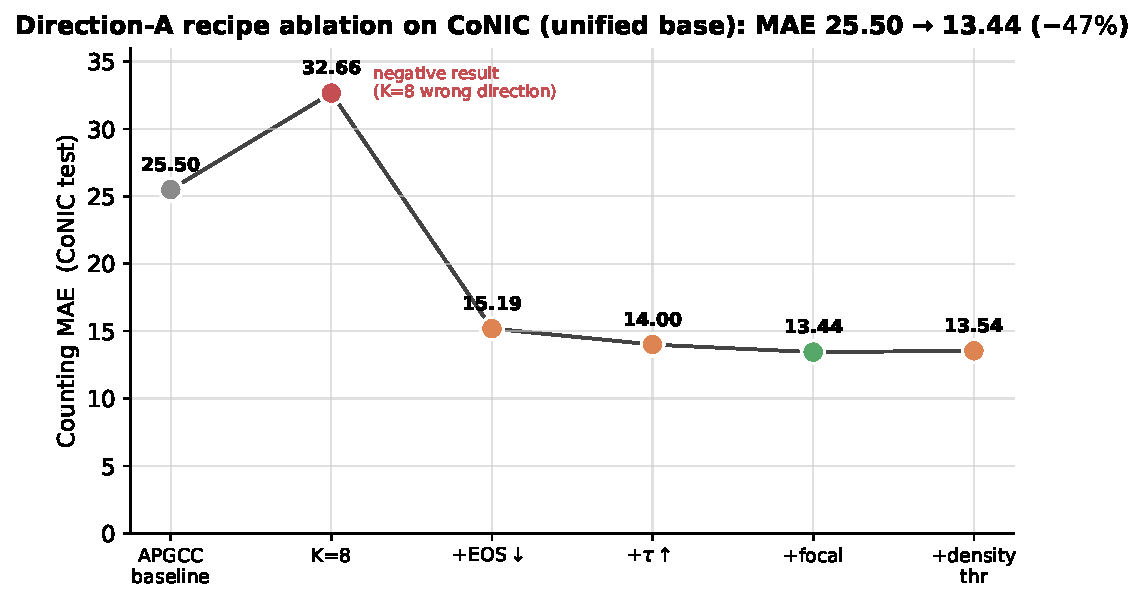
\includegraphics[width=0.82\linewidth]{figures/fig_A_ablation}
    \caption{方向 A 在 CoNIC（unified 基座）上的配方逐步消融（均为最终 val-best 检查点）。灰点为 baseline，
    红点为 $K{=}8$ 负结果，绿点为最优配方；MAE 由 $25.50$ 降至 $13.44$（$-47\%$），主要由 EOS/$\tau$ 贡献。}
    \label{fig:A-ablation}
\end{figure}

\paragraph{机理特异性：配方精准修复"少计"，对其它失败模式中性。}
为验证该配方是\emph{对症}而非碰运气，方向 A 在三个数据集上各自训练并对比（表~\ref{tab:A-transfer}、
图~\ref{fig:A-transfer}）。结果与各数据集的失败模式高度吻合：CoNIC（密集少计）大幅获益（$25.50\to14.00$）；
BCData（计数平衡）近似中性（$17.19\to18.35$）；MoNuSeg（整体过计）近似中性（$26.21\to24.79$）。
即该配方只在"少计"这一失败模式上显著生效，对"平衡"和"过计"模式不强行改变，符合其机理设计。

\begin{table}[H]
    \centering
    \caption{方向 A 配方的三数据集机理特异性迁移（各自训练）}
    \label{tab:A-transfer}
    \small
    \begin{tabular}{lcccc}
        \toprule
        数据集 & 失败模式 & baseline MAE & +配方 MAE & 结论 \\
        \midrule
        CoNIC   & 密集少计 & 25.50 & 14.00 & 大幅获益 \\
        BCData  & 平衡     & 17.19 & 18.35 & 近似中性 \\
        MoNuSeg & 过计     & 26.21 & 24.79 & 近似中性 \\
        \bottomrule
    \end{tabular}
\end{table}

\begin{figure}[H]
    \centering
    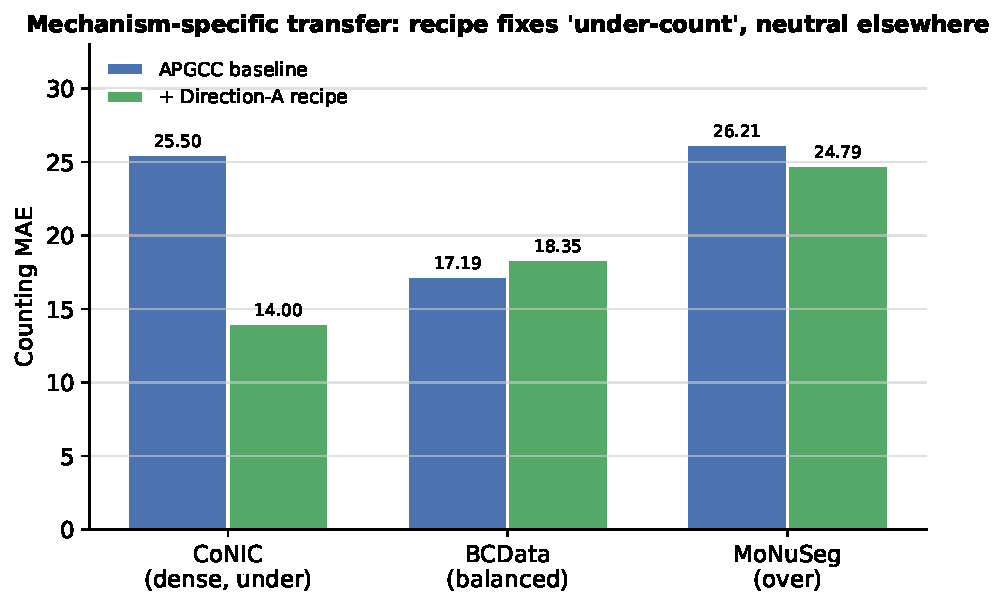
\includegraphics[width=0.74\linewidth]{figures/fig_A_transfer}
    \caption{方向 A 配方在三数据集上的迁移。仅 CoNIC（密集少计）显著获益，BCData/MoNuSeg 近似中性，
    印证配方对"少计"失败模式的针对性。}
    \label{fig:A-transfer}
\end{figure}

\paragraph{基座依赖性：native 是最终落地基座，校准价值正比于基座标定误差。}
方向 A 的最终落地基座是\emph{原生增强（native）}——团队后续所有改进与集成均在 native 上进行，
统一增强（unified）仅作为"增广敏感性 / 机理验证"的对照保留。两套增强对 CoNIC 的影响差异巨大：
unified 严重伤害 CoNIC（unified baseline MAE $25.50$，而统一 native baseline 仅 $12.93$，相差近一倍），
其根源是 unified 把置信度分布推向严重欠预测，而 native 基座本身已较平衡（计数偏差约 $-5.5\%$）。
因此本文把方向 A 的\emph{完整 EOS$\times\tau$ 与 focal 扫描}放在 native 基座上、并\emph{训练至收敛}
（ep$\ge$120）后报告，结果见表~\ref{tab:A-native} 与图~\ref{fig:A-native}。

native 上的扫描呈现三点与 unified \emph{相反}的规律。其一，所有配方的 MAE 都落在 $10.5$--$16.3$、
与统一 native baseline（$12.93$）处于同一量级，没有 unified 上那种量级改善。其二，最优方向与 unified 完全相反——
native 上 EOS 越低越差（$0.25\!\to\!10.83$，$0.10\!\to\!12.50$，$0.05\!\to\!16.31$），而 unified 上恰是
EOS 越低越好；$\tau$ 过大（$0.15$）同样劣化。其三，就真正关心的定位 F1 而言，\emph{统一 baseline 的 $0.7929$
即为全表最佳，没有任何 A 配方能超过它}（最接近的 EOS$0.25/\tau0.10$ 也仅 $0.78$ 量级）；尤其
EOS$0.10/\tau0.05$ 虽在低阈值（$0.1$）下取得全表最低 MAE $10.54$，但其 F1 仅 $0.7185$，说明该点是靠
\emph{正负误差相消}得到的好计数、定位质量反而最差——只看单一 MAE 会产生误导。focal 在 native 同样无益（$12.15$）。
综合 MAE 与 F1：native 上 A 配方至多在计数上与 baseline 互有胜负，但\emph{定位始终不及 baseline}，整体呈中性偏弱。

由此得到方向 A 的核心结论：\emph{置信度与匹配校准的价值，正比于基座本身的标定错误程度}。在标定很差的
unified 基座上，校准把 MAE 从 $25.50$ 拉到 $\approx13.4$（$-47\%$，转化巨大）；而在标定良好的 native 基座上，
同类校准增益显著温和、远小于 unified（图~\ref{fig:A-native} 右），且定位 F1 始终不及 baseline。两基座上最优超参方向相反，
恰恰说明该方法是\emph{对症校准}而非偶然调参——native 基座已经"健康"，可校准的空间本就很小。

\begin{table}[H]
    \centering
    \caption{方向 A 在 native（最终落地）基座上的 EOS$\times\tau$ 与 focal 完整扫描
    （CoNIC 测试集，均训练至 ep$\ge$120 收敛；阈值取各配置 MAE 甜点）。baseline 行采用\emph{团队统一 native
    baseline}（CoNIC 方向E 口径，MAE $12.93$/F1 $0.7929$），与各 A 配置非同次运行，故 MAE 的细微差异含运行间方差，
    \emph{稳健结论以定位 F1 为准}（无 A 配置超过 baseline）。}
    \label{tab:A-native}
    \small
    \begin{tabular}{lcccccl}
        \toprule
        native 配置 & 阈值 & MAE$\downarrow$ & MSE$\downarrow$ & F1@12$\uparrow$ & 计数偏差 & 备注 \\
        \midrule
        baseline（统一口径）           & 0.50 & 12.93 & 468.9  & \textbf{0.7929} & $-5.5\%$ & 团队统一 native baseline（定位最优） \\
        EOS0.25/$\tau$0.10             & 0.40 & 10.83 & 396.9  & 0.7810 & $-1.3\%$ & native MAE 最优 \\
        \quad（同配置 @0.50）           & 0.50 & 11.12 & 438.8  & 0.7799 & $-4.6\%$ & 阈值敏感性对照 \\
        EOS0.10/$\tau$0.05             & 0.10 & \textbf{10.54} & 251.6 & 0.7185 & $-0.6\%$ & 低阈值，F1 最差 \\
        EOS0.10/$\tau$0.10             & 0.70 & 12.50 & 537.1  & 0.7309 & $-2.8\%$ & $\approx$\,baseline \\
        EOS0.10/$\tau$0.15             & 0.80 & 15.10 & 398.8  & 0.7402 & $-8.5\%$ & $\tau$ 过大变差 \\
        EOS0.05/$\tau$0.10             & 0.70 & 16.31 & 1004.3 & 0.6840 & $-3.8\%$ & EOS 过低变差 \\
        +\,focal (EOS0.10/$\tau$0.10)  & 0.60 & 12.15 & 563.3  & 0.7740 & $-7.0\%$ & focal 无益 \\
        \bottomrule
    \end{tabular}
\end{table}

\begin{figure}[H]
    \centering
    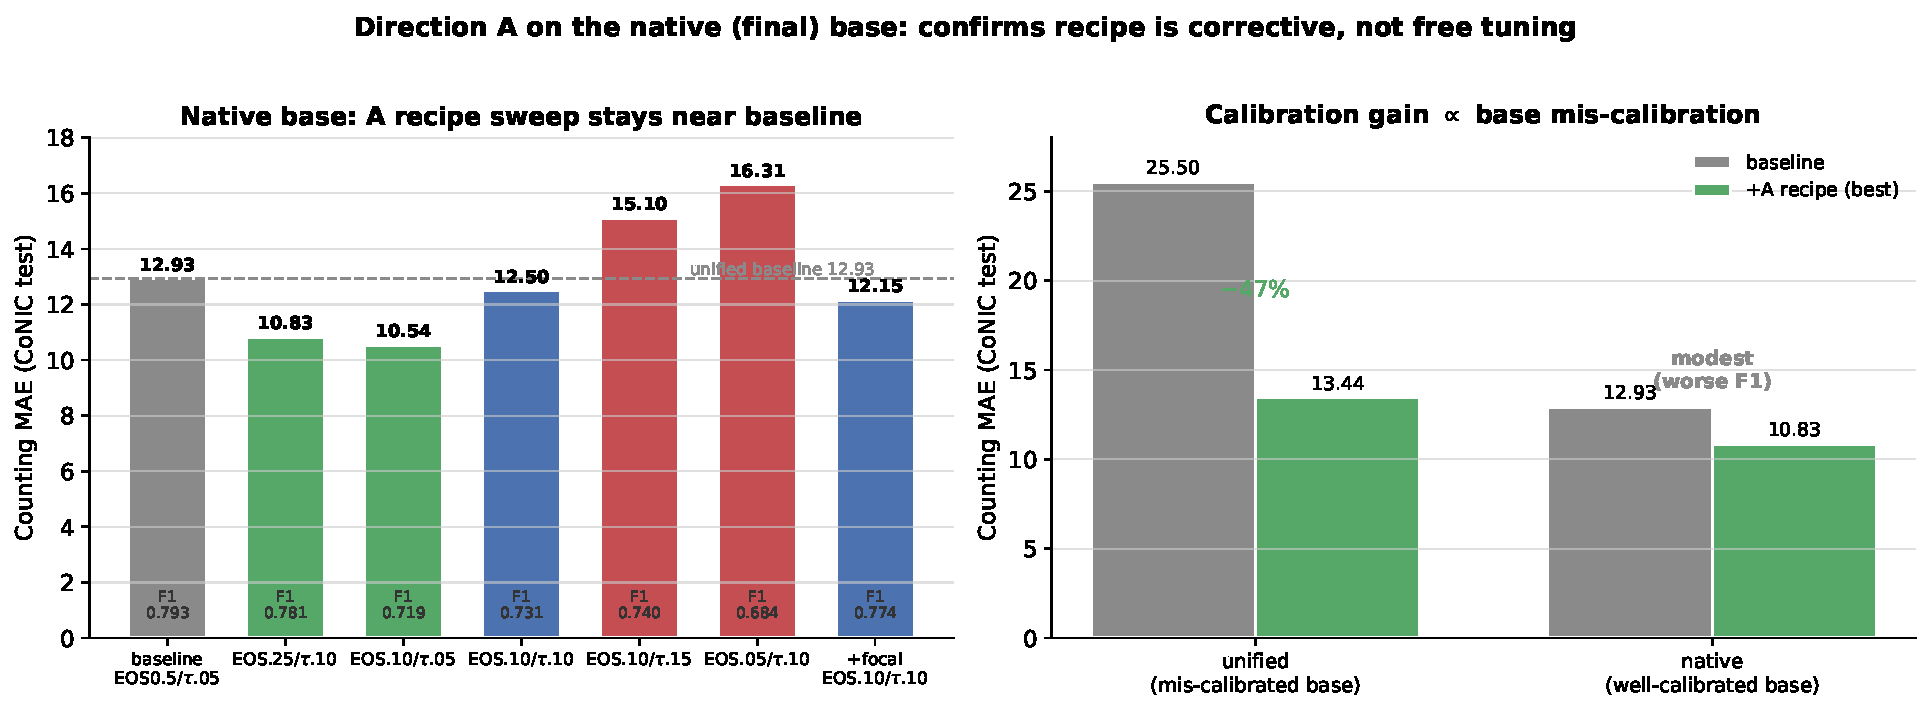
\includegraphics[width=\linewidth]{figures/fig_A_native}
    \caption{方向 A 在 native（最终落地）基座上的结果。左：EOS$\times\tau$ 与 focal 的完整扫描，
    各配方 MAE 与统一 native baseline（$12.93$）同量级、定位 F1 均不超过 baseline，且最优方向与 unified 相反；
    右：native 与 unified 的校准增益对比——unified（烂基座）转化巨大（$-47\%$），native（好基座）增益温和，
    印证"校准价值正比于基座标定误差"。}
    \label{fig:A-native}
\end{figure}

\paragraph{小结。}
方向 A 通过"先诊断、后对症"的方式，否定了直觉性的加参考点（$K{=}8$）方案，定位到匹配争用与类别不平衡
两个真因，提出 EOS$\downarrow$+$\tau\uparrow$（+focal/密度自适应）的组合校准。在标定很差的 unified 基座上，
该校准取得 MAE $25.50\to\approx13.4$（$-47\%$，主要由 EOS/$\tau$ 贡献）、计数偏差由 $-21.7\%$ 收敛到近平衡的显著改善，
作为机理验证；而在团队\emph{最终落地的 native 基座}上，由于统一 baseline（$12.93$）本身已较平衡，同类校准增益温和
（无配方在 F1 上超过 baseline、MAE 也与 baseline 同量级），最优超参方向且与 unified 完全相反。两者共同支撑方向 A 的核心结论：\emph{置信度与匹配校准是针对"少计"失败模式的
对症方法，其收益正比于基座标定误差}——这也解释了为何后续集成（见 ADE）中 A 的贡献应落在\emph{后处理校准}、
而非训练配方。
